\documentclass[conference]{IEEEtran}
\IEEEoverridecommandlockouts
\usepackage{biblatex}
\usepackage{amsmath,amssymb,amsfonts}
\usepackage{algorithmic}
\usepackage{graphicx}
\usepackage{textcomp}
\usepackage{xcolor}
\usepackage{enumitem}

\addbibresource{ROB_Projekt.bib}

\begin{document}

\title{Haptisches Feedback eines Roboters durch virtuelle 3D-Modelle}

\author{
    \IEEEauthorblockN{Carl Gathmann}
    \IEEEauthorblockA{\textit{Universität zu Lübeck}\\
        Lübeck, Germany \\
        carl.gathmann@student.uni-luebeck.de}
    \and
    \IEEEauthorblockN{Marten Buchmann}
    \IEEEauthorblockA{\textit{Universität zu Lübeck}\\
        Lübeck, Germany \\
        marten.buchmann@student.uni-luebeck.de}
}
\maketitle

\begin{abstract}
!!!NOCH GPT!!!
In dieser Studie wird ein Ansatz zur Generierung von haptischem Feedback in Mensch-Roboter-Interaktionen vorgestellt. Mittels maßgeschneiderter Software erzeugen wir eine sensorische Wahrnehmung, die durch frei gestaltbare, virtuelle 3D-Modelle gesteuert wird. Der Anwender erfährt eine Art abweisende Kraft, die durch die räumlichen Grenzen des virtuellen Modells definiert ist, wodurch eine physische Interaktion mit dem immateriellen Modell simuliert wird. Die vorgestellte Technologie findet breite Anwendungsbereiche, von medizinischen Simulationen und Exploration in gefährlichen Zonen bis hin zur Erhöhung der Spielerfahrung in virtuellen Umgebungen. In Verbindung mit Virtual-Reality-Ausrüstung eröffnet unsere Methode neue Wege zur Verbesserung der Benutzerimmersion durch die Vermittlung eines realistischeren Gefühls für die Form und Textur virtueller Objekte. Die in dieser Arbeit vorgestellten Prinzipien und Implementierungen können als Grundlage für weiterführende Forschungen und Entwicklungen auf diesem aufstrebenden Gebiet dienen.
\end{abstract}

\begin{IEEEkeywords}
    component, formatting, style, styling, insert
\end{IEEEkeywords}

\section{Einleitung}
!!! GPT =>

Die Mensch-Roboter-Interaktion hat in den letzten Jahren zunehmend an Bedeutung gewonnen und sich als ein dynamisches Forschungs- und Anwendungsfeld etabliert. Im Zentrum dieser Interaktion steht die Verbesserung der Benutzererfahrung durch die Erweiterung der sinnlichen Wahrnehmung des Menschen.

In dieser Studie präsentieren wir einen Ansatz, der es dem Benutzer ermöglicht, virtuelle 3D-Modelle zu "ertasten", indem er über ein Roboterinterface mit ihnen interagiert. Dies wird durch die Erzeugung einer abweisenden Kraft erreicht, die auf den Grenzen der virtuellen Modelle basiert. Dieses haptische Feedback simuliert das physische Berühren eines realen Objekts, obwohl kein tatsächlicher physischer Kontakt mit dem virtuellen Modell besteht. 

Dieser Ansatz bietet zahlreiche Anwendungsmöglichkeiten, darunter die Simulation von Operationen für Ausbildungszwecke, die Erkundung von Objekten in gefährlichen oder unzugänglichen Umgebungen und die Erhöhung der Immersion in virtuellen Spielen. Darüber hinaus kann die Kombination unserer Technologie mit Virtual-Reality-Brillen zu einem verbesserten Gefühl von Präsenz und Realismus in virtuellen Umgebungen führen.

Das vorliegende Paper beleuchtet die zugrundeliegenden Prinzipien, technische Details und potenzielle Anwendungen dieses Ansatzes.

<= GPT !!!

\section{Methods}
Die Erzeugung des haptischen Feedbacks beruht auf der Berechnung einer abweisenden Kraft, die so konzipiert ist, dass dem Benutzer ein realistisches Gefühl für die Form des virtuellen 3D-Modells vermittelt wird. Die Modelle können als Datei im STL-Standart übergeben werden. Der STL-Standart speichert 3D-Modelle als Dreiecksmesh, das aus Eckpunkten und den Normalen der Dreiecke besteht. Es ist keine besondere CAD Software nötig um 3D-Modelle im STL Format zu erstellen. Außerdem ist das Format weit verbeitet und wird in der Industire zur Speicherung und Übertragung von 3D-Modellen eingesetzt. Das sorgt für hohe Flexibilität 
und einfache Handhabung. !!!Quelle zu STL Standart!!!

Für die physische Implementierung der Mensch-Roboter-Interaktion wurde der Panda-Roboter von Franka Emika ausgewählt. Der Panda zeichnet sich durch seine 7-achsige Struktur aus, die hohe Präzision und Flexibilität bietet. Eine benutzerfreundliche, 3D-gedruckte Schnittstelle (siehe \ref{fig:MRinterface}) wurde am Endeffektor des Roboters installiert, um die Führung durch menschliche Benutzer zu erleichtern.  

\begin{figure}
    \centering
    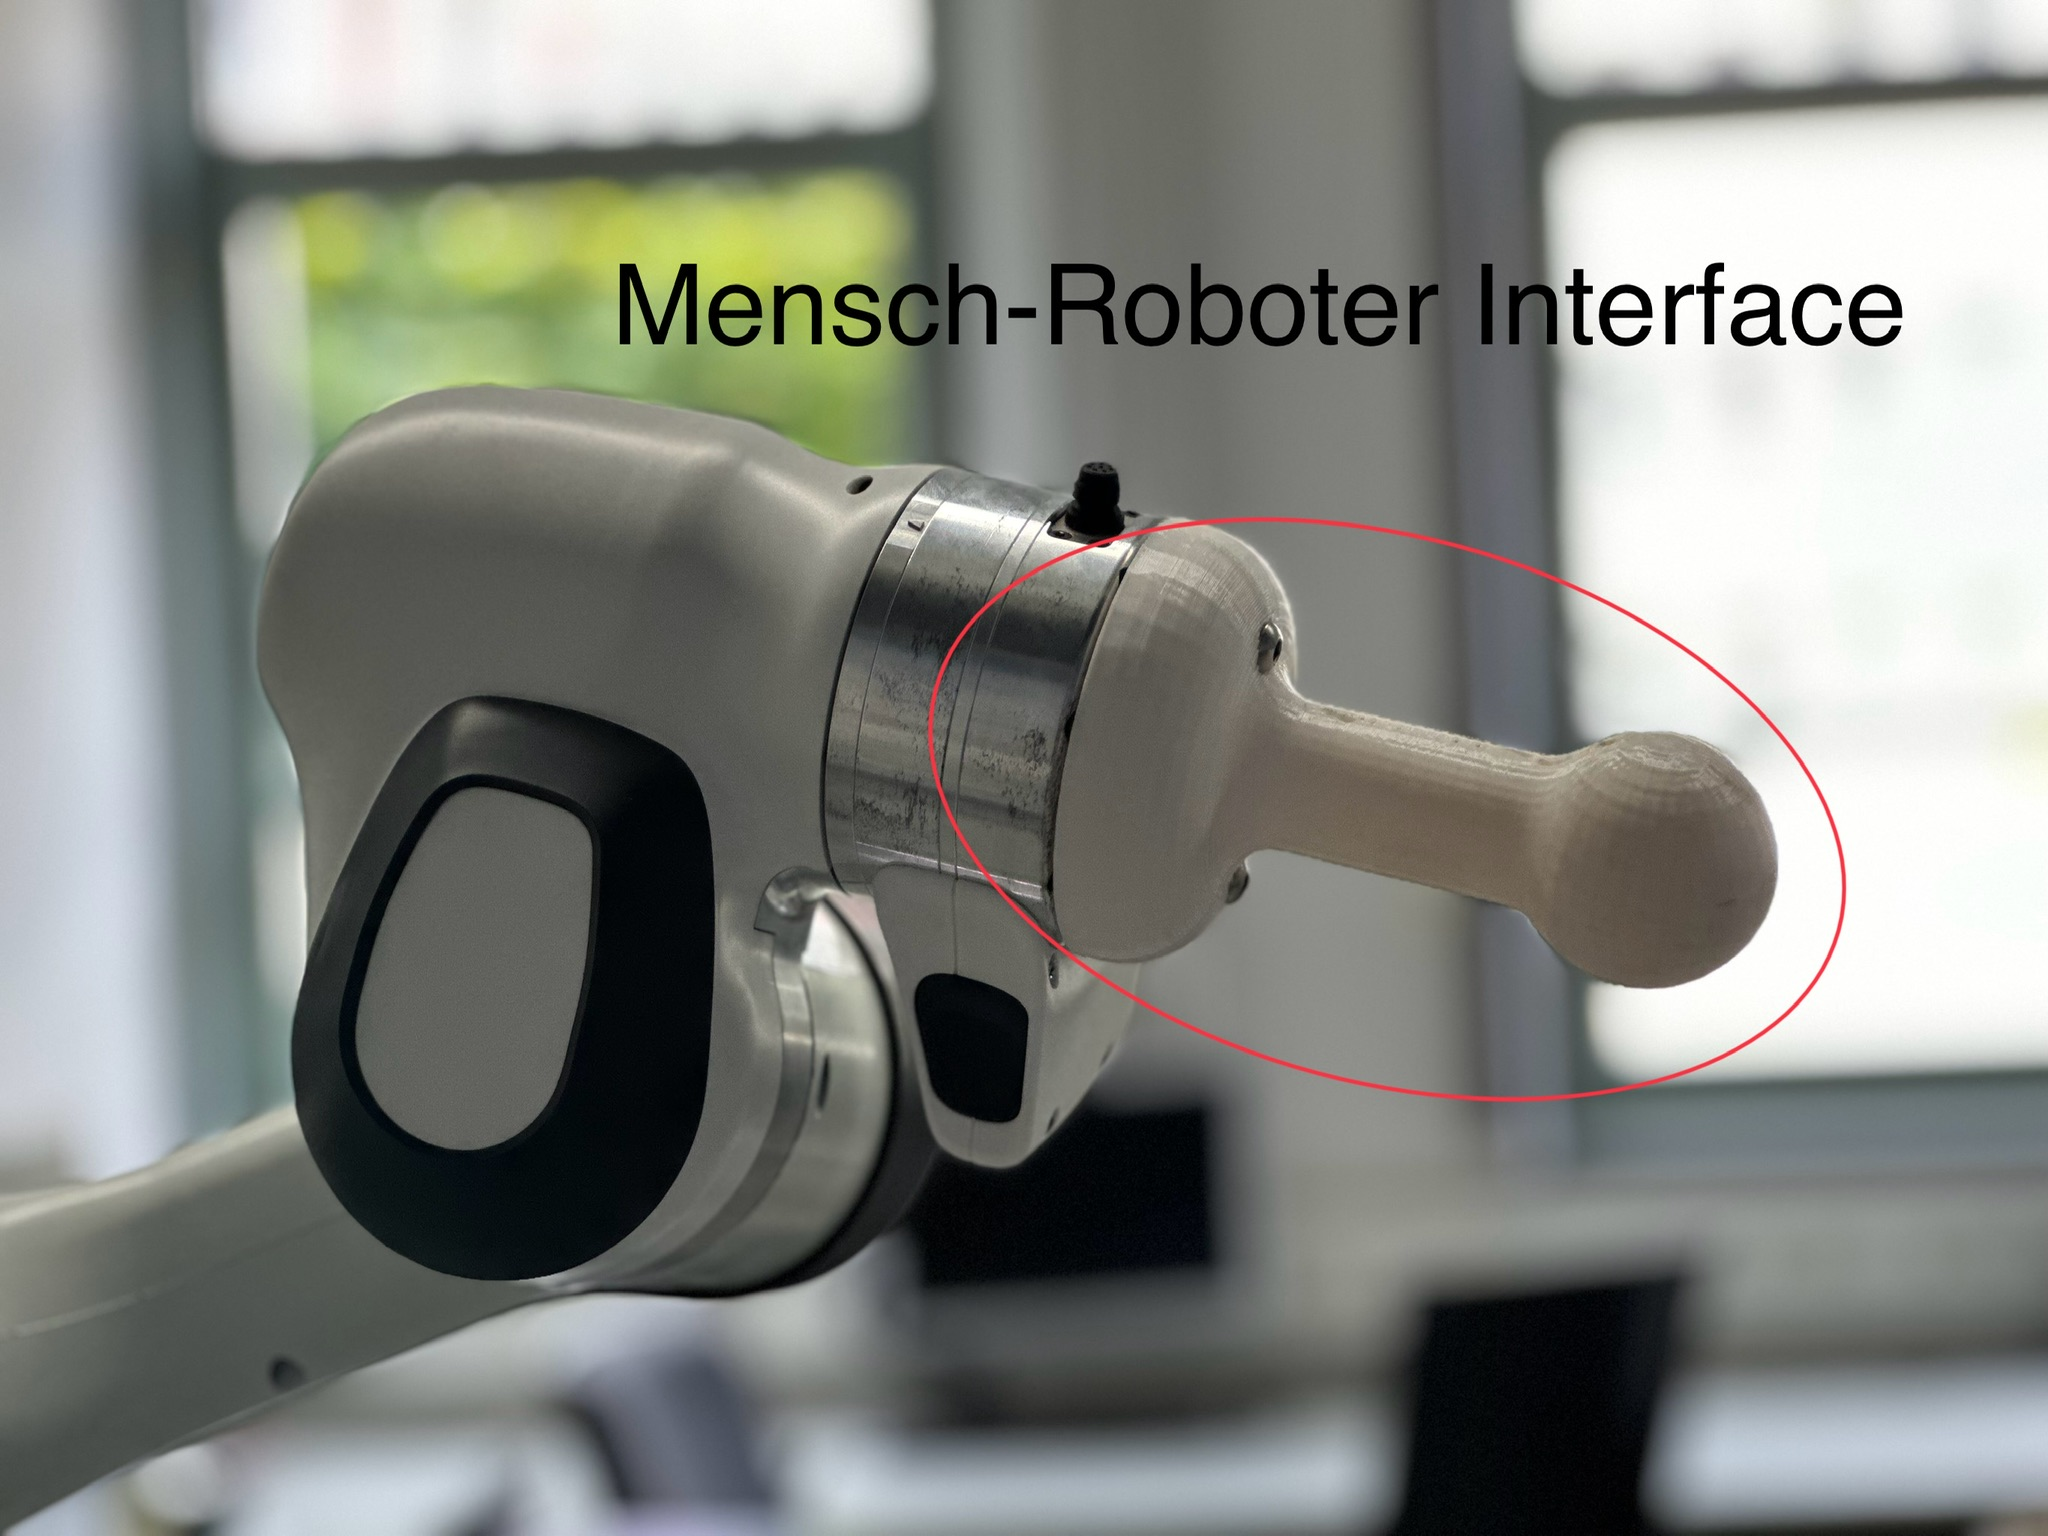
\includegraphics[width=0.45\textwidth]{pics/interface.jpeg}
    \caption{Mensch-Roboter-Schnittstelle}
    \label{fig:MRinterface}
\end{figure}

Bei der Entwicklung der Software für dieses System stand die Leistungsfähigkeit im Vordergrund, um eine nahtlose Benutzererfahrung zu gewährleisten. Dazu war es entscheidend, dass die Anwendung in Echtzeit ausgeführt werden kann, wobei eine maximale 
Zeitverzögerung von weniger als 1 Millisekunde akzeptiert wurde. Die Programmiersprache 
C++ wurde aufgrund ihrer hohen Performance ausgewählt, um diesem Anspruch gerecht zu werden. 
Die Hardware-Konfiguration bestand aus !!!HARDWARE!!!.
Die Verarbeitung und Nutzung der 3D-Modelle wurden durch die Umwandlung der STL-Daten in 
Eigen-Matrizen optimiert. Für diesen Prozess wurde durch einen STL-Parser benutzt. Dadurch ist eine einfache und effiziente Handhabung der 3D-Daten innerhalb des Programms möglich.

Während der Recherche des Projekts wurden verschiedene Ansätze zur Erzeugung der abstoßenden Kraft, welche in den folgenden Abschnitten vorgestellt werden.

Als Vorbereitung auf die Verwendung der Ansätze \ref*{edge} und \ref*{bary} muss zuerst ein zweidimensionales Problem aus dem dreidimensionalen Problem gemacht werden. Erreicht wird dies durch die Erstellung eines neuen Koordinatensystems für jedes Dreieck, welches sich ergibt durch:
\begin{enumerate}
    \item Eine Kante des Dreiecks als x-Achse
    \item Das Kreuzprodukt der entstandenen Achse mit einem weiteren Vektor als z-Achse
    \item Das Kreuzprodukt der beiden entstandenen Achsen als y-Achse
\end{enumerate}
Die Koordinaten des Punktes werden dann in diesem Koordinatensystem angegeben. Auf diese Art 
repräsentieren die x- und y-Koordinaten die Position und die z-Koordinate die Entfernung des Punktes 
von der Ebene des Dreiecks. 

\subsection{Edge Funktion}\label{edge}
Die Edge-Funktion ist eine häufig verwendete Funktion im Bereich der Computer-Grafik. Sie wird 
verwendet, um herauszufinden, wo sich ein Punkt relativ zu einem Dreieck befindet. Definiert ist 
sie wie folgt:
\begin{equation}
    E_{i} = (x_{i+1} - x_{i})(y - y_{i}) - (y_{i+1} - y_{i})(x - x_{i})
\end{equation}
x, y sind die Koordinaten des Punktes, $x_{i}$, $y_{i}$ sind die Koordinaten des i-ten Eckpunktes 
des Dreiecks.
Im Fall eines Dreiecks mit den Eckpunkten $A$, $B$ und $C$ und einem Punkt $P$ ist der Punkt innerhalb 
des Dreiecks, wenn gilt:
\begin{equation}
    E_{AB} \geq 0 \land E_{BC} \geq 0 \land E_{CA} \geq 0
\end{equation}

!!!BILD!!!

Mit dem Wissen, ob ein Punkt innerhalb des Dreiecks liegt und der Höhe des Punktes, die über 
die z-Koordinate des transformierten Punktes gegeben ist, kann ein Kraftvektor berechnet werden. 
Dieser Kraftvektor zeigt in Richtung der Normalen des Dreiecks und ist proportional zur Höhe des Punktes. 
Die Kraft kann dann wie folgt berechnet werden:
\begin{equation}
    F = \frac{1}{z} \cdot n
\end{equation}
$z$ ist die z-Koordinate des Punktes, der innerhalb des Dreiecks liegt und $n$ ist die Normale dieses Dreiecks.
Die großen Vorteile dieser Methode sind die Einfachheit und die Geschwindigkeit. 
Die Berechnung der Edge-Funktion ist sehr einfach und schnell, bietet aber keine Möglichkeit, zwischen den einzelnen Dreiecken zu interpolieren. Daher enstehen Unstetigkeiten an den Kanten der Dreiecke, was zu unintuitivem und sprunghaftem Verhalten führen kann, wenn der Benutzer sich entlang der Kante 
bewegt. Aus diesem Grund haben wir die Methode verworfen und uns an einer weiteren Methode versucht.

\subsection{Baryzentrische Koordinaten} \label{bary}
Eine weitere Methode, die wir untersucht haben, ist die Verwendung von baryzentrischen Koordinaten. 
Diese Methode ist sehr ähnlich zur Edge-Funktion, da sie auch verwendet wird, um herauszufinden, 
wo sich ein Punkt relativ zu einem Dreieck befindet. Ein wichtiger Unterschied ist allerdings, dass außerdem die relative Position innerhalb des Dreiecks bestimmt werden kann. Berechnet werden die Koordinaten wie folgt:
\begin{equation*}
    \lambda_b = \pm\frac{|\Lambda(\triangle(Q,B,C))|}{|\Lambda(\triangle(A,B,C))|}
\end{equation*}
\begin{equation}
    \lambda_c = \pm\frac{|\Lambda(\triangle(A,Q,C))|}{|\Lambda(\triangle(A,B,C))|}
\end{equation}
\begin{equation*}
    \lambda_a = 1 - \lambda_1 - \lambda_2
\end{equation*}
A, B, C sind hierbei die Eckpunkte des Dreiecks und P die in das Koordinatensystem des Dreiecks transformierte Roboter Position. $\Lambda$ repräsentiert eine Funktion für den Flächeninhalt eines Dreiecks. $\lambda_1$, $\lambda_2$ und $\lambda_3$ sind die baryzentrischen Koordinaten des Punktes P, welche aussagen, wie weit der Punkt von den jeweiligen Eckpunkten entfernt ist. 
Wenn alle drei Koordinaten positiv sind, liegt der Punkt innerhalb des Dreiecks. Nun lässt sich ein 
Schwellwert festlegen, ab dem eine Interpolation zwischen den Kanten/Eckpunkten des Dreiecks stattfindet. 
Dazu ist es notwendig, für jede Kante zu wissen, welche Dreiecke sie enthält und welche Normalen diese 
Dreiecke haben. Das Gleiche gilt für die Eckpunkte. Anschließend kann die Kraft wie folgt 
berechnet werden:
\begin{equation*}
    F_{BC} = 
    \begin{cases} 
        \frac{\lambda_a}{S}\cdot N_{\triangle} + (1-\frac{\lambda_a}{S})\cdot N_{BC} &  0 < \lambda_a < \text{S} \\
        0 & \text{sonst.}
    \end{cases}
\end{equation*}
\begin{equation*}
    F_{AC} = 
    \begin{cases} 
        \frac{\lambda_b}{S}\cdot N_{\triangle} + (1-\frac{\lambda_a}{S})\cdot N_{AC} &  0 < \lambda_b < \text{S} \\
        0 & \text{sonst.}
    \end{cases}
\end{equation*}
\begin{equation*}
    F_{AB} = 
    \begin{cases} 
        \frac{\lambda_c}{S}\cdot N_{\triangle} + (1-\frac{\lambda_a}{S})\cdot N_{AB} &  0 < \lambda_c < \text{S} \\
        0 & \text{sonst.}
    \end{cases}
\end{equation*}
$N_{\triangle}$ ist dabei die Normale des betrachteten Dreiecks und $N_{XY}$ sind dabei die Normalen der Dreiecke, die die jeweilige Kante XY enthalten. $S$ ist ein Benutzerdefinierter Schwellwert, ab dem die Interpolation stattfindet.
Die resultierende Kraft $F_{XY}$ ist die Kraft, die auf den Benutzer wirkt, wenn er sich auf der Kante zwischen den Punkten X und Y bewegt.

Für die Eckpunkte gilt ein ähnlicher Ansatz. Entsprechend wird die Kraft wie folgt berechnet:
\begin{equation*}
    F_{A} = 
    \begin{cases} 
        (1-\frac{\lambda_a}{S})\cdot N_{\triangle} + \frac{\lambda_a}{S}\cdot N_{A} &  S < \lambda_a < 1 \\
        0 & \text{sonst.}
    \end{cases}
\end{equation*} 
\begin{equation*}
    F_{B} = 
    \begin{cases} 
        (1-\frac{\lambda_b}{S})\cdot N_{\triangle} + \frac{\lambda_b}{S}\cdot N_{B} &  S < \lambda_a < 1 \\
        0 & \text{sonst.}
    \end{cases}
\end{equation*} 
\begin{equation*}
    F_{C} = 
    \begin{cases} 
        (1-\frac{\lambda_c}{S})\cdot N_{\triangle} + \frac{\lambda_c}{S}\cdot N_{C} &  S < \lambda_a < 1 \\
        0 & \text{sonst.}
    \end{cases}
\end{equation*} 
Der Vorteil gegenüber der Edge-Funktion ist, dass so die Unstetigkeit entlang der Kanten vermieden wird, 
die Berechnung der baryzentrischen Koordinaten ist jedoch etwas komplexer und langsamer als die 
Berechnung der Edge-Funktion. Daher wurde auch diese Variante letztendlich nicht verwendet.

\subsection{Point-Triangle-Distance-Funktion}
Die tatsächlich angewandte Methode zur des Kraftvektors basiert auf den Untersuchungen von \Citeauthor{DistancePointTriangle}. Diese  präsentieren eine Methode zur Berechnung der Punkt-Dreieck-Distanz und liefern dabei zwei wesentliche Werte zurück:

\begin{enumerate}
\item 'dist': Dieser Parameter repräsentiert den minimalen Abstand zwischen einem vorgegebenen Punkt 'p' und dem Dreieck. Der Wert entspricht der kürzesten euklidischen Distanz, die von 'p' bis zur nächsten Position auf dem Dreieck (seien es Kanten, Eckpunkte oder eine Flächenposition innerhalb der Dreiecksgrenzen) gemessen wird.
\item 'pp0': Dieser Parameter repräsentiert den entsprechenden Punkt auf dem Dreieck, der 'p' am nächsten liegt. Es handelt sich hierbei um den Punkt auf dem Dreieck, der den minimalen Abstand 'dist' zu 'p' aufweist.
\end{enumerate}

Die Berechnungsmethode beruht auf der Anwendung von Vektoren und Skalarprodukten und integriert speziell die Berücksichtigung verschiedener 'Regionen'. Diese 'Regionen' sind durch die relativen Positionen des Punktes 'p' und des Dreiecks definiert und erlauben eine effiziente Bestimmung des kürzesten Abstandes und des nächstgelegenen Punktes auf dem Dreieck. Die genaue Definition und Charakterisierung dieser 'Regionen' kann aus \ref{fig:regions} entnommen werden.

Die Anwendung dieser Methode ermöglicht somit eine präzise und effiziente Bestimmung der Punkt-Dreieck-Distanz im dreidimensionalen Raum.

\begin{figure}[h]
    \centering
    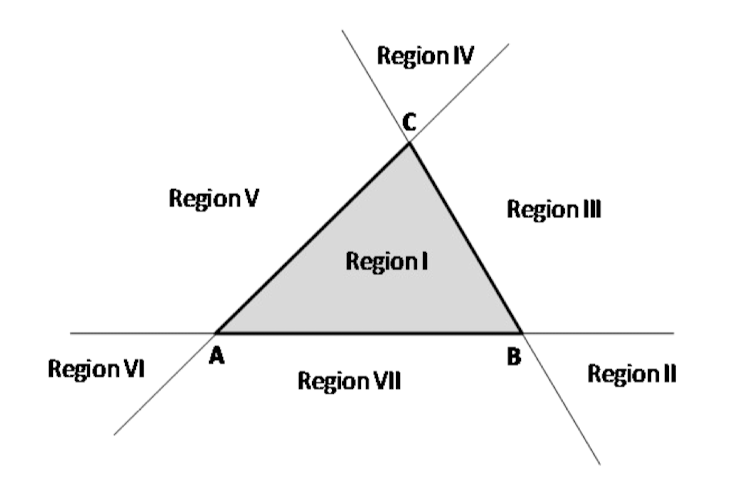
\includegraphics[width=0.5\textwidth]{pics/regions.png}
    \caption{Die verschiedenen Regionen, die durch die relative Position des Punktes und des Dreiecks definiert sind \cite{regionen}.}
    \label{fig:regions}
\end{figure}
\begin{samepage}
    Um den resultierenden Kraftvektor zu ermitteln, wurde folgendes Verfahren implementiert: \\
    \textbf{für jedes Dreieck der STL Datei:}
    \begin{enumerate}
        \item Berechnung von $dist$ und $pp0$ mit Hilfe der Point-Triangle-Distance-Funktion.
        \item Berechnung des Vektors $v$ zwischen $pp0$ und der Roboterposition $p$.
        \item Wenn das Skalarprodukt von $v$ und der Normalen des Dreiecks positiv ist, wird die resultierende Kraft um
        \begin{equation*}
            F \mathrel{+}= v * f(dist)
        \end{equation*}
        ergänzt. 
    \end{enumerate}
    Die Funktion $f(dist)$ ist dabei eine linear fallende Funktion, die den Einfluss der Distanz auf die Kraft bestimmt.
\end{samepage}

\begin{figure}[h]
    \centering
    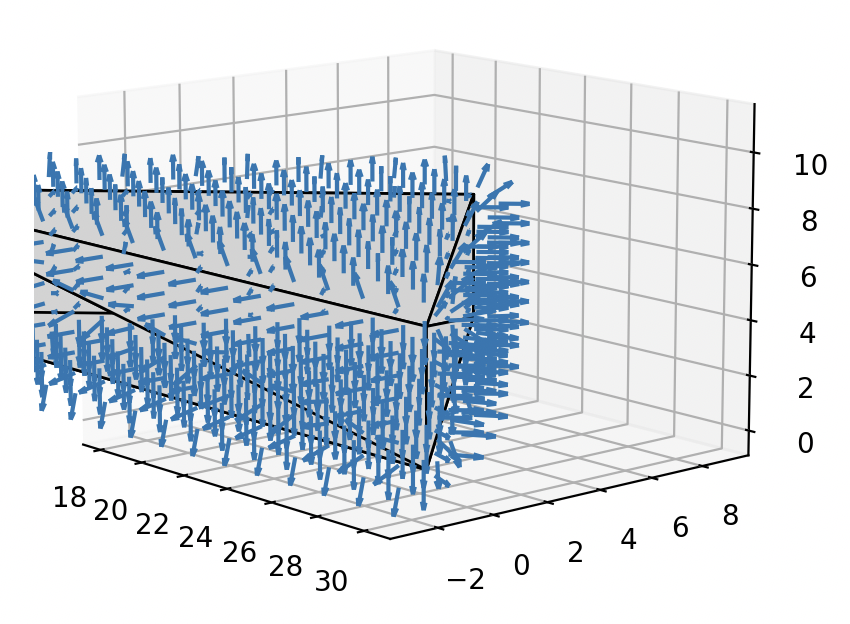
\includegraphics[width=0.5\textwidth]{pics/vectorfield.png}
    \caption{Vektorfeld, das resultierende Kräfte für verschiedene Punkte visualisiert.}
    \label{fig:vectorfield}
\end{figure}

Zur Visualisierung der Kräfte für verschiedene Punkte wurde ein Vektorfeld erstellt (siehe \ref{fig:vectorfield}). Man kann klar erkennen, dass keine Unstetigkeiten entlang der Kanten und Eckpunkten auftreten.


\section{Ergebnisse}

\subsection{Effekt}
Bei der Überprüfung unserer Implementierung konnten wir feststellen, dass der beabsichtigte Effekt der abstoßenden Kraft sowie das gewünschte Gefühl von Plastizität erfolgreich erreicht wurden. Die Kanten und Ecken der in der STL-Datei definierten Struktur waren deutlich wahrnehmbar. Ein kurzes Demonstrationsvideo, welches die Funktionsweise und das Resultat der angewandten Implementierung veranschaulicht, kann unter dem folgenden Link eingesehen werden:
\begin{minipage}{\textwidth}
    \nobreak\url{https://youtu.be/IhARjkxuTvw}.
\end{minipage}

\subsection{Performanz}
Hinsichtlich der Performance wurden ebenfalls zufriedenstellende Resultate erzielt. Bei der Verarbeitung einer STL-Datei, welche 160 Dreiecke beinhaltet, betrug die durchschnittliche Berechnungszeit für den Kraftvektor eines Punktes lediglich 0.714 Millisekunden bei der oben beschriebenen Hardware. Im Kontext einer Echtzeitanwendung stellt dieser Wert eine akzeptable Berechnungslast dar. 

\section{Discussion}
Sollten die STL-Dateien jedoch eine bestimmte Größe überschreiten und es und es wird keine leistungsfähigere Hardware eingesetzt, könnte die Anforderung an die Echtzeitfähigkeit nicht mehr zuverlässig erfüllt werden. Eine potenzielle Lösung hierfür könnte die Anwendung von Level of Detail (LOD) Modellen sein. Diese Modelle, die bei größerer Entfernung des Roboters zum Objekt genutzt werden können, zeichnen sich durch eine reduzierte Anzahl an Dreiecken aus und können demzufolge effizienter verarbeitet werden. Auch die Nutzung von Octrees könnte die Performance weiter verbessern, da durch deren Einsatz die Anzahl der zu verarbeitenden Dreiecke verringert werden kann. Ein Octree ist eine spezielle Art von Baumstruktur, die im Kontext der 3D-Computergrafik verwendet wird und eine effiziente räumliche Aufteilung ermöglicht. Durch die Anwendung dieser Methoden könnte die Leistungsfähigkeit des Systems auch bei umfangreicheren STL-Dateien erhalten bleiben und die Echtzeitanforderungen sicherstellen.

\section{Conclusion}

\printbibliography

\end{document}